% Copyright 2004 by Till Tantau <tantau@users.sourceforge.net>.
%
% In principle, this file can be redistributed and/or modified under
% the terms of the GNU Public License, version 2.
%
% However, this file is supposed to be a template to be modified
% for your own needs. For this reason, if you use this file as a
% template and not specifically distribute it as part of a another
% package/program, I grant the extra permission to freely copy and
% modify this file as you see fit and even to delete this copyright
% notice. 

\documentclass[8pt]{beamer}

% There are many different themes available for Beamer. A comprehensive
% list with examples is given here:
% http://deic.uab.es/~iblanes/beamer_gallery/index_by_theme.html
% You can uncomment the themes below if you would like to use a different
% one:
%\usetheme{AnnArbor}
%\usetheme{Antibes}
%\usetheme{Bergen}
%\usetheme{Berkeley}
%\usetheme{Berlin}
%\usetheme{Boadilla}
%\usetheme{boxes}
%\usetheme{CambridgeUS}
%\usetheme{Copenhagen}
%\usetheme{Darmstadt}
%\usetheme{default}
%\usetheme{Frankfurt}
%\usetheme{Goettingen}
%\usetheme{Hannover}
%\usetheme{Ilmenau}
%\usetheme{JuanLesPins}
%\usetheme{Luebeck}
\usetheme{Madrid}
%\usetheme{Malmoe}
%\usetheme{Marburg}
%\usetheme{Montpellier}
%\usetheme{PaloAlto}
%\usetheme{Pittsburgh}
%\usetheme{Rochester}
%\usetheme{Singapore}
%\usetheme{Szeged}
%\usetheme{Warsaw}
%\usepackage{amsmath}
%\usepackage{algorithm}
%\usepackage{algpseudocode}
\usepackage{marvosym}
\usepackage{tikzsymbols}
\usepackage{textcomp}
\usepackage{parskip}

%\usepackage{pifont}
%\usepackage{float}
%\floatplacement{figure}{H}

%\usepackage{subcaption}

\setbeamerfont{institute}{size=\fontsize{7pt}{7pt}}
\setbeamerfont{author}{size=\fontsize{7pt}{8pt}}
\setbeamerfont{date}{size=\fontsize{7pt}{8pt}}
\setbeamerfont{title}{size=\fontsize{11pt}{12pt}}
\setbeamerfont{caption}{size=\small}
%\setbeamerfont{subsection}{size=\tiny}
\setbeamertemplate{caption}{\raggedright\insertcaption\par}
\makeatletter
\setbeamertemplate{footline}
{
  \leavevmode%
  \hbox{%
  \begin{beamercolorbox}[wd=.333333\paperwidth,ht=2.25ex,dp=1ex,center]{author in head/foot}%
    \usebeamerfont{author in head/foot}\insertsection
  \end{beamercolorbox}%
  \begin{beamercolorbox}[wd=.333333\paperwidth,ht=2.25ex,dp=1ex,center]{title in head/foot}%
    \usebeamerfont{title in head/foot}\insertsubsection
  \end{beamercolorbox}%
  \begin{beamercolorbox}[wd=.333333\paperwidth,ht=2.25ex,dp=1ex,right]{date in head/foot}%
    \usebeamerfont{date in head/foot}\insertshortdate{}\hspace*{2em}
    \insertframenumber{} / \inserttotalframenumber\hspace*{2ex} 
  \end{beamercolorbox}}%
  \vskip0pt%
}


\makeatother

\makeatletter

\setbeamertemplate{title page}
{
\bigskip
\begin{frame} 
\centering
    \begin{beamercolorbox}[sep=8pt,center,shadow=true,rounded=true]{title}
      \usebeamerfont{title}\inserttitle\par%
    \end{beamercolorbox}%
   \newline
   \small
  {\centering\itshape part of \par}
  \newline
  \large
  {\centering \insertsubtitle \par}
    \vskip0.2em\par
    \begin{beamercolorbox}[sep=8pt,center]{date}
      \usebeamerfont{date}\insertdate
    \end{beamercolorbox}%\vskip0.5em
    \begin{beamercolorbox}[sep=8pt,center]{author}
      \usebeamerfont{author}\insertauthor
    \end{beamercolorbox}
  \end{centering}
  %\vfill
  \end{frame}
  
}
\makeatother


\title{Autonomous UAV Navigation in Unknown Indoor Environment using Onboard Light Weight Camera}
% A subtitle is optional and this may be deleted
\subtitle{TRADR - Teaming for Robot-Assisted Disaster Response}
\date{28th April 2015}
\author{Devvrat Arya\\ Masters in Autonomous System\\
  Hochshule Bonn Rhein Sieg}
% - Give the names in the same order as the appear in the paper.
% - Use the \inst{?} command only if the authors have different
%   affiliation.\setbeamerfont{author}{size=\small}

\institute[Hochshule Bonn Rhein Sieg] % (optional, but mostly needed)
{
  Intelligent Analysis and Information Systems \\
  Fraunhofer IAIS, Sankt Augustin}
% - Use the \inst command only if there are several affiliations.
% - Keep it simple, no one is interested in your street address.


% - Either use conference name or its abbreviation.
% - Not really informative to the audience, more for pe\fiople (including
%   yourself) who are reading the slides online

\subject{}
% This is only inserted into the PDF information catalog. Can be left
% out. 

% If you have a file called "university-logo-filename.xxx", where xxx
% is a graphic format that can be processed by latex or pdflatex,
% resp., then you can add a logo as follows:

% \pgfdeclareimage[height=0.5cm]{university-logo}{university-logo-filename}
% \logo{\pgfuseimage{university-logo}}


% Delete this, if you do not want the table of contents to pop up at
% the beginning of each subsection:
\iffalse 
\AtBeginSubsection[]
{
  \begin{frame}<beamer>{Outline}
    \tableofcontents[currentsection,currentsubsection]
  \end{frame}
}
\fi

% Let's get started

\begin{document}

\begin{frame}
  \titlepage
{\centering\itshape Supervisors:\par}
\begin{center}
{\fontsize{7pt}{8pt}
\begin{tabular}[t]{@{}l@{\hspace{3pt}}p{.32\textwidth}@{}}
&\textbf{Dr. rer. nat. Bj\"{o}rn Kahl}\\
&Hochshule Bonn Rhein Sieg\\
&Sankt Augustin, Germany.\\
&bjoern.kahl@h-brs.de	
\end{tabular}%
\begin{tabular}[t]{@{}l@{\hspace{3pt}}p{.32\textwidth}@{}}
&\textbf{Mr. Rainer Worst}\\
&Fraunhofer- IAIS\\
&Sankt Augustin, Germany.\\
&rainer.worst@iais.fraunhofer.de
\end{tabular}}%
\end{center}
\end{frame}

\begin{frame}{Contents}
  \tableofcontents[hideallsubsections]
  % You might wish to add the option [pausesections]
\end{frame}

% Section and subsections will appear in the presentation overview
% and table of contents.
\section{Introduction}

\subsection{Motivation}

\begin{frame}{Motivation}%{optional subtitle}
  \begin{itemize}
  \setlength\itemsep{2em}
  %\item {To minimize the impact of Natural disasters on human life and livelihood.}
  \item{Recognize the scope and extent of the disaster damage over the affected area.}
  \item{Robots and UAVs can be of great help to analyze the scene.}
  \item{This can help to most effectively begin rescue and disaster recovery activities.}
  \end{itemize}
\end{frame}

\begin{frame}{Motivation}
  \begin{itemize}
  \setlength\itemsep{1em}
  \item {
    Functioning in collapsed building, requires robot to traverse cluttered and uneven environment.%\pause % The slide will pause after showing the first item
  }
  \item {Ground robot can traverse rough terrain but in terrains with levels it is not physically capable.}
 \item {UAV is an alternative robotic platform for rescue tasks and a host of other applications.}
  % You can also specify when the content should appear
  % by using <n->:
  %\item<3-> {UAV is an alternative robotic platform for rescue tasks and a host of other applications.
  %}
  %\item<4-> {
   % Fourth item.
  %}
  % or you can use the \uncover command to reveal general
  % content (not just \items):
  %\item<5-> {
  %  Fifth item. \uncover<6->{Extra text in the fifth item.}
  %}
  \end{itemize}
  \begin{figure}[h]
  \centering
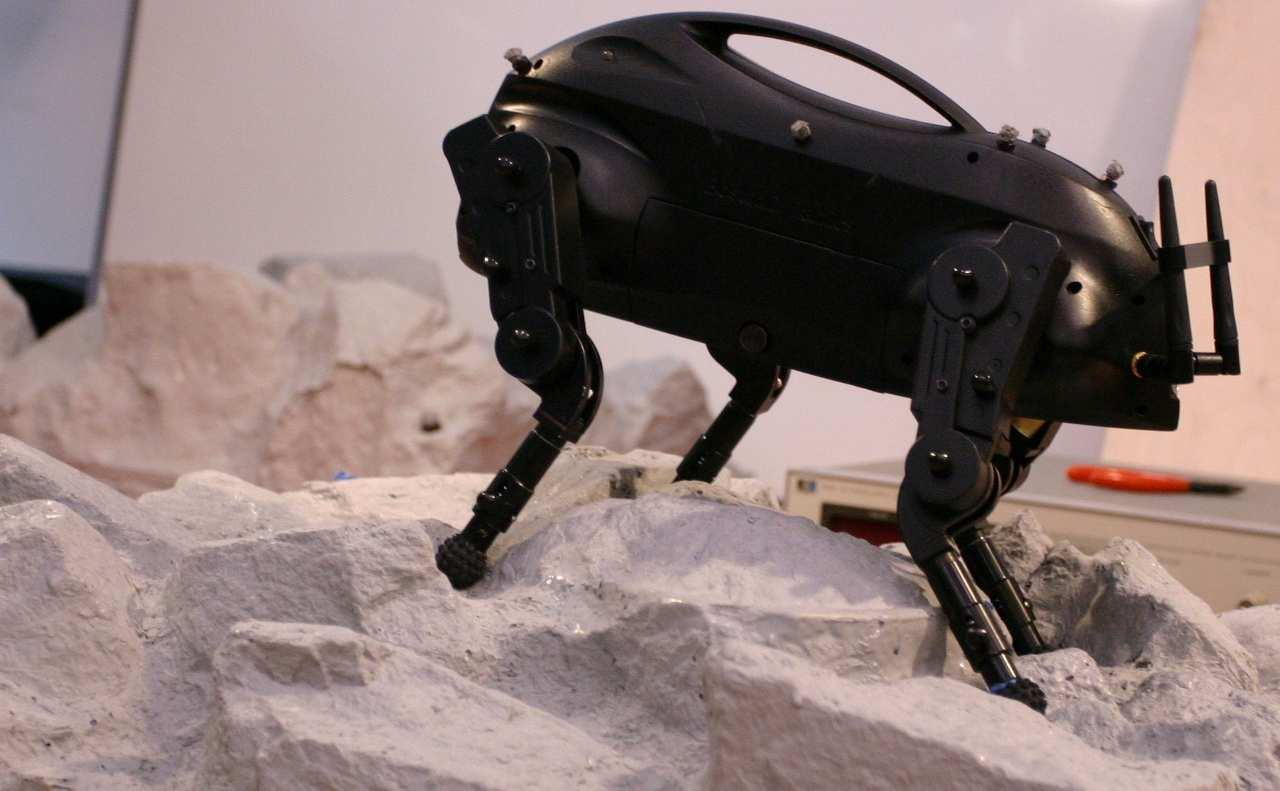
\includegraphics[width=4cm, height=3cm]{images/groundrobot1.jpeg}%
\hspace{1cm}
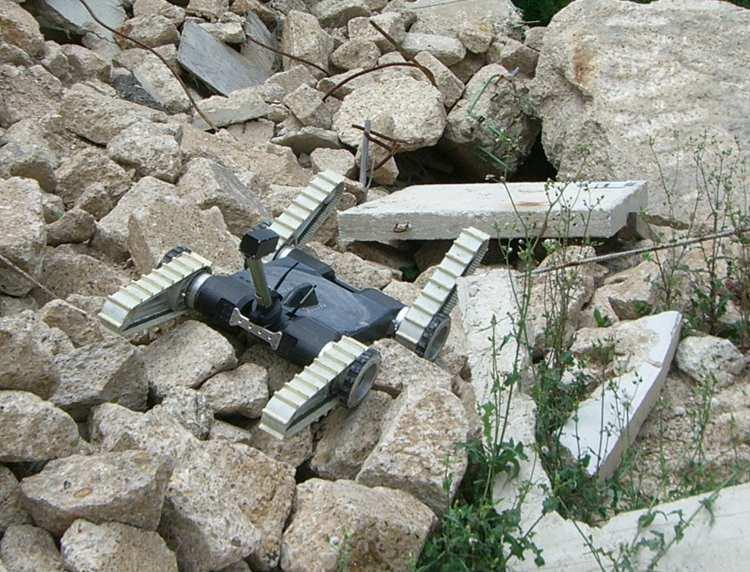
\includegraphics[width=4cm, height=3cm]{images/groundrobot2.jpeg}%
\caption{Ground robots that can traverse through rough surfaces}%
  \label{fig:ground_robots}
\end{figure}
\end{frame}

\subsection{Objective}
% You can reveal the parts of a slide one at a time
% with the \pause command:
\begin{frame}{Objective}
  Constraints with UAVs:
  \begin{itemize}
  \setlength\itemsep{1em}
  \item {Payload %\pause % The slide will pause after showing the first item
  }
  \item {Computational limitations}
 \item {Fast dynamics}
  \end{itemize}
  \bigskip
  \textit{The objective of this R\&D is to design and implement a basic navigation system for UAVs
  which uses only on-board light weight camera, requires minimum computation and less power consuming.}  
\end{frame}
\iffalse{
\section{Constraints with UAVs}
\begin{frame}{Constraints with UAVs}
  \begin{itemize}
   \setlength\itemsep{2em}
    \item {Payload}
    \begin{itemize}
    \setlength\itemsep{1em}
     \item {Equip UAVs with maximum useful and necessary sensors under limited payload.}
     \item {UAVs must be small and lightweight. Passive, long-range, low power consuming sensor is preferable.}
    \end{itemize} 
  \item {Computational limitations}
  \begin{itemize}
  \setlength\itemsep{1em}
     \item {Mounted processor on embedded systems like UAV is less powerful.}
     \item {Navigation algorithms are computationally demanding even for powerful desktop computers.}
    \end{itemize}
 \item {Fast dynamics}
 \begin{itemize}
 \setlength\itemsep{1em}
     \item {Movement of UAV is not steady as ground vehicle.}
     \item {All quantities necessary to stabilize the vehicle should be computed fast.}
    \end{itemize}
  \end{itemize}
\end{frame}
}
\fi


\section{Related Work}

\subsection{Related Work}

\begin{frame}{Related Work}
\begin{itemize}
\setlength\itemsep{2em}
\item {Non Vision sensors based indoor UAV navigation:}
    \begin{itemize}
    \setlength\itemsep{1em}
      \item Kumar \& Ghose and Kwag \& Kang implemented radar based
	    navigation and obstacle avoidance.
      \item Saunders used a forward looking laser range finder for
	    path planning. 
    \end{itemize}
    \bigskip
  \textit{
    \alert{These approaches lack in heavy weight or high power consumption.}}
\item {Vision sensors based Unknown indoor UAV navigation:}
    \begin{itemize}
    \setlength\itemsep{1em}
      \item Saxena and Courbon used vision to fly in known environments based on visual databases.
      \item Chao, Yu Gu and Napolitano presented optical flow techniques for UAV navigation.
      \item Conte and Patrick used inertial sensors and visual odometry.
    \end{itemize}
    \bigskip
  \textit{
    \alert{These approaches would not apply in many indoor environments that are devoid of
track-able features.}}
\end{itemize}
\end{frame}


\section{Problem handled}

%\section*{Constraint}
\subsection{How to handle computational limitations?}
% You can reveal the parts of a slide one at a time
% with the \pause command:
\begin{frame}{How to handle computational limitations?}
\begin{itemize}[<+(1)->]
 \setlength\itemsep{1em}
     \item<+(1)-> {Receive data from environment sensors(Motion trackers or camera) and UAV(IMU).}
     \item<+(1)-> {Run autonomy algorithms(navigation algorithms) on external system(desktop computers).}
     \item<+(1)-> {Send navigation commands back to UAV}
    \end{itemize}
 \begin{figure}[h]
  \centering
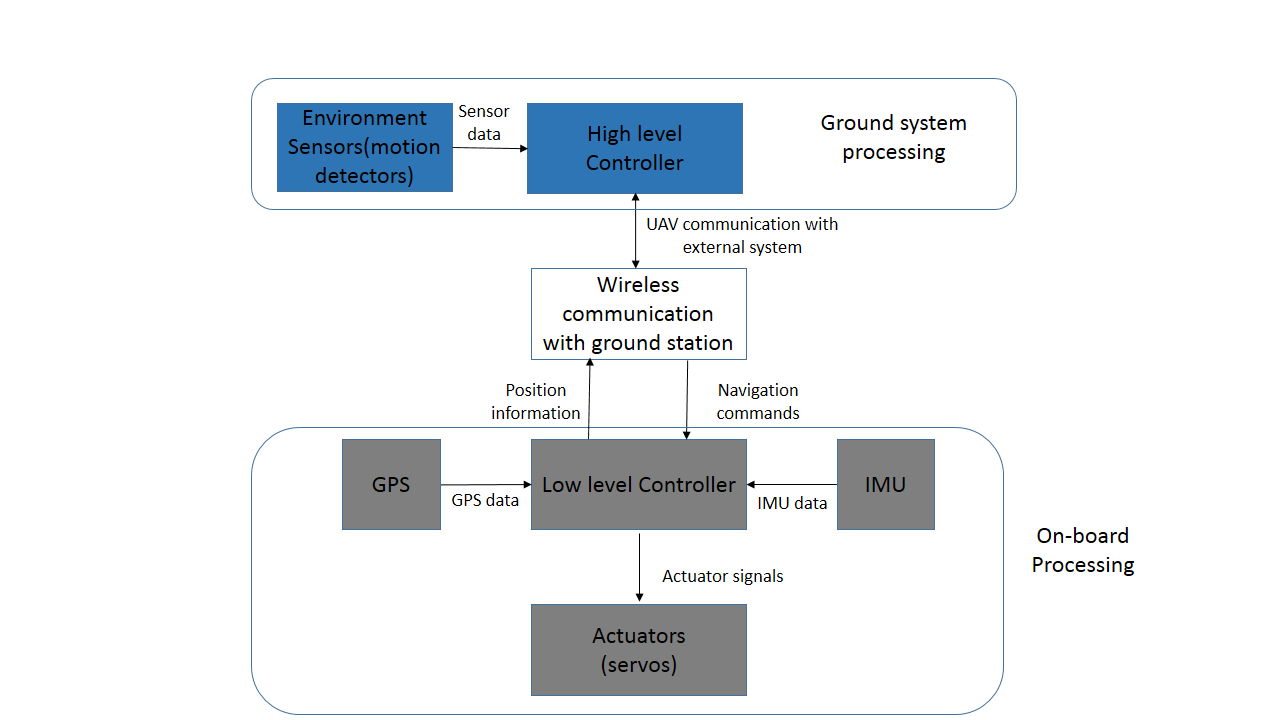
\includegraphics[width=10cm]{images/basic_acrh2.PNG}%
\caption{Basic drone architecture with computation on ground system}%
  \label{fig:drone_ground_communication}
\end{figure}
  
\end{frame}

\begin{frame}{How to handle computational limitations?}
\begin{itemize}
 \setlength\itemsep{1em}
     \item {Receive sensor data(image cues) from UAV.}
     \item {Run autonomy algorithms(navigation algorithms) on external system(desktop computers).}
     \item {Send navigation commands back to UAV}
    \end{itemize}
 \begin{figure}[h]
  \centering
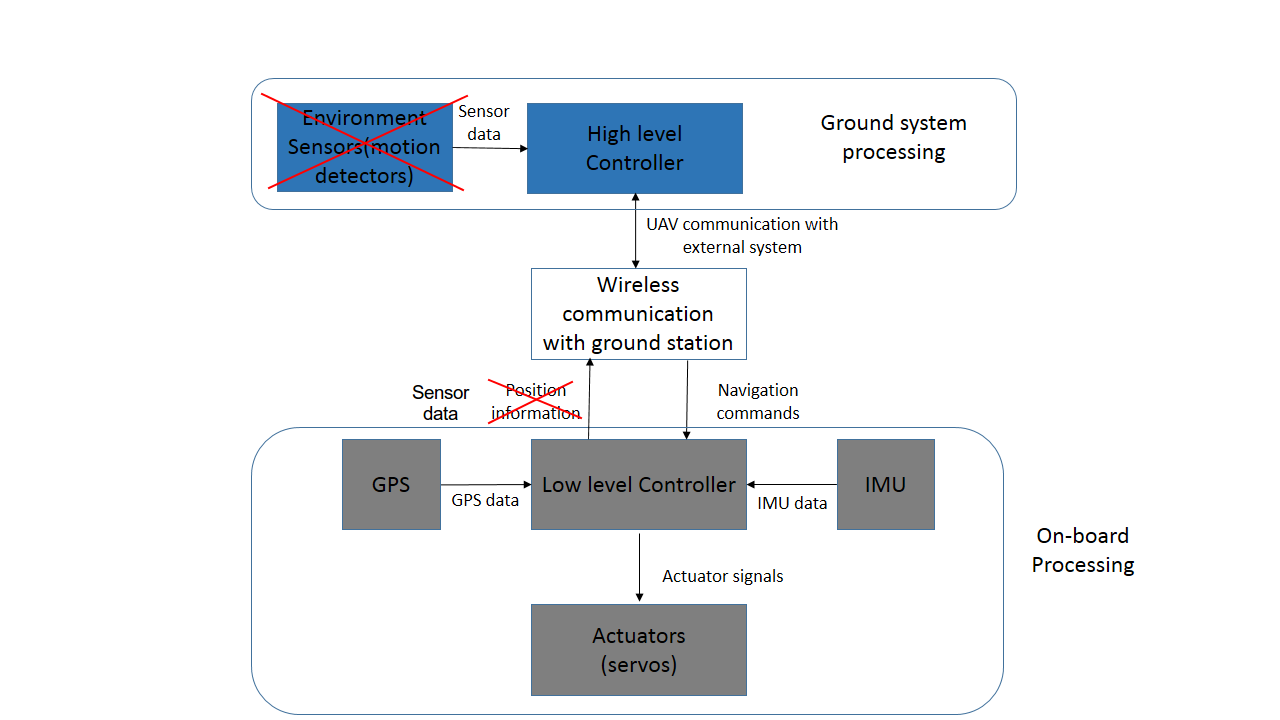
\includegraphics[width=10cm]{images/basic_acrh2_2.PNG}%
\caption{Basic drone architecture with computation on ground system}%
  \label{fig:drone_ground_communication}
\end{figure}
  
\end{frame}

\begin{frame}{Problem handled}
Design and implement a navigation system prototype for UAV which: 
\bigskip
  \begin{itemize}%[<+(1)->]
    \setlength\itemsep{1em}
    \item enables a UAV to autonomously explore corridor environments
    \item uses only on-board sensors and works without prior knowledge of the environment
    \item less computationally expensive (algorithm able to run onboard)
    \item based on simple features extraction
    \item suited for long-term navigation.
  \end{itemize}
  
  \begin{figure}[h]
  \centering
    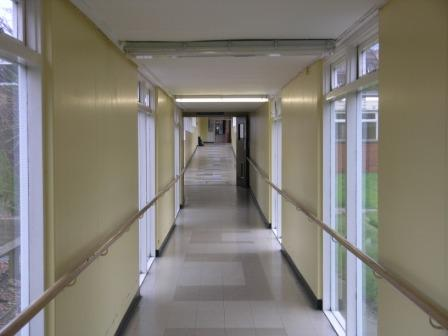
\includegraphics[width=3cm, height=3cm]{images/corridor1.jpg}%
    \hspace{0.3cm}
    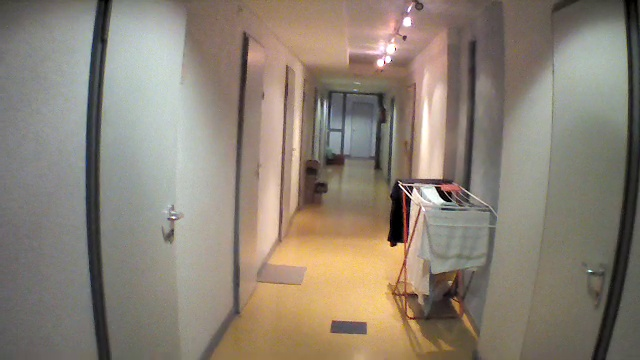
\includegraphics[width=3cm, height=3cm]{images/corridor2.jpg}%
    \hspace{0.3cm}
    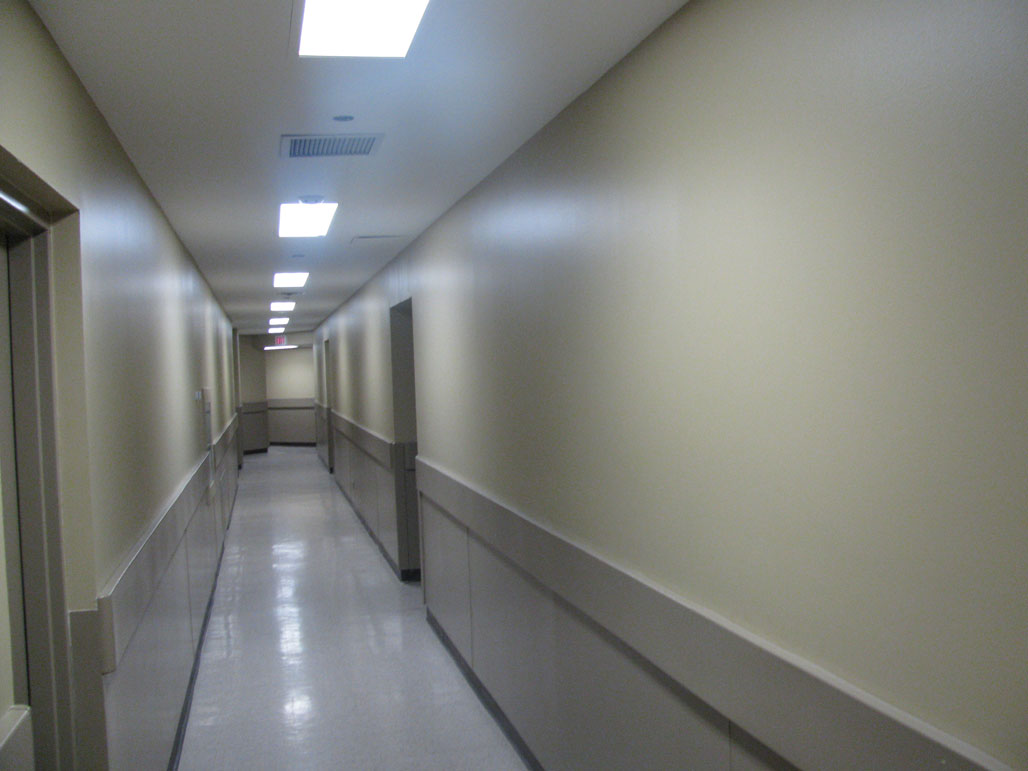
\includegraphics[width=3cm, height=3cm]{images/corridor3.jpg}%
    \caption{Corridor sample images}
    \label{Figure: corridor_sample_images}%
\end{figure}
  
\end{frame}


\section{Setup and Platform}

\begin{frame}{Setup and Platform}
Primary platform is the Parrot AR.Drone 2.0 quadrotor: 
\bigskip
  \begin{itemize}
    \setlength\itemsep{1em}
    \item first implement our approach on the Parrot A.R. Drone
    \item less computational capabilities on-board, therefore computation happens on ground system
    \item algorithm runs on host machine \textendash Lenovo Y560 (Intel\textregistered Core i7 CPU Q720@1.60GHzx8, 4GB RAM), running Ubuntu 12.04
    \item commands and images are exchanged via WiFi between host machine and AR.Drone
  \end{itemize}
\vspace{0.5cm}
\textit{If successful, implement the approach on \textbf{AscTec Pelican quadrotor}, TRADR project target platform.
AscTec Pelican has computational power similar to our host machine.}


\end{frame}

\begin{frame}{Setup and Platform}

\begin{columns}[c]
    \column{0.5\textwidth}
        \begin{figure}
            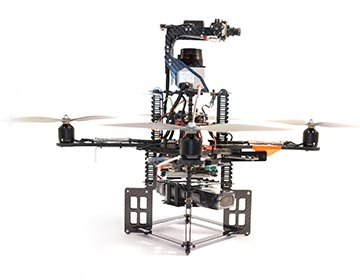
\includegraphics[width=3cm, height=3cm]{images/AscTec_pelican.jpg}%
	    \caption{AscTec Pelican}
	    \label{Figure: AscTec_Pelican}%
        \end{figure}
        \footnotesize{
	  \begin{table}[h]
	  \centering
	  \begin{tabular}{@{}ll@{}}
	  \hline
	  \multicolumn{2}{c}{Technical Data – AscTec Pelican} \\
	  \hline
	  UAV Type & Quadcopter  \\
	  Onboard computer & Up to 3rd Generation\\
	  ~&Intel\textregistered Core i7 processor \\
	  Size & 700 x 700 x 500 mm  \\
	  Max. take off weight & 1,65 kg\\ 
	  Max. payload & 650 g \\
	  Flight time incl. payload & 16 min.\\
	  Wireless communication & 2,4 GHz XBee link\\
	  Sensors & HD Camera, \\
	  ~ & Hokuyo laser scanner,...\\
	  \end{tabular}
	  \end{table}
	 }
        
    \column{0.5\textwidth}
        \begin{figure}
             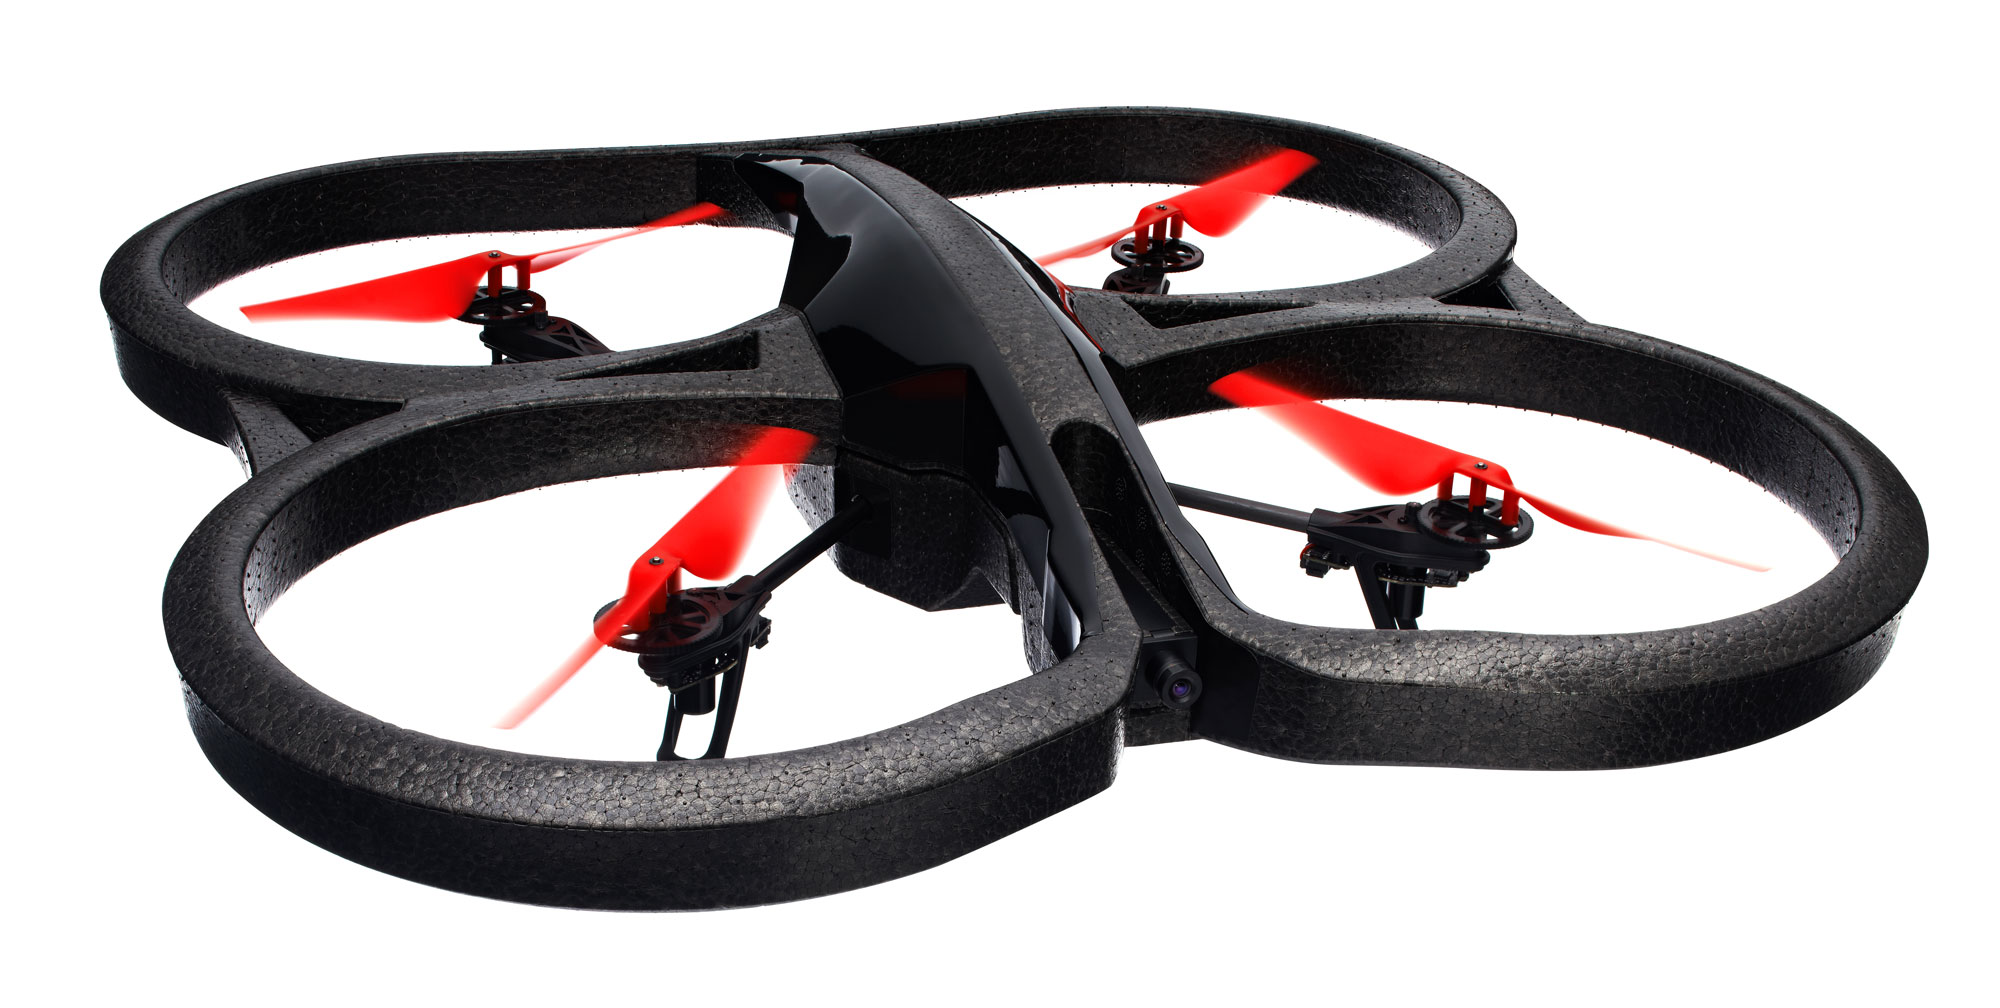
\includegraphics[width=3cm, height=3cm]{images/AR_Drone_2.jpg}%
	     \caption{Parrot AR.Drone 2.0}
	     \label{Figure: Parrot_AR_Drone_2}%
        \end{figure}     
        \footnotesize{
	  \begin{table}[h]
	  \centering
	  \begin{tabular}{@{}ll@{}}
	  \hline
	  \multicolumn{2}{c}{Technical Data – Parrot AR Drone 2} \\
	  \hline
	  UAV Type & Quadcopter  \\
	  Onboard computer & 1 GHz ARM \\
	  ~ & Cortex-A8 CPU\\
	  Size & 670 x 670 x 125 mm  \\
	  Max. take off weight & 380grams\\ 
	  Max. payload & 250grams(unstable)\\
	  Flight time incl. payload & 15 min.\\
	  Wireless communication & 802.11n WiFi\\
	  Sensors & Front HD 720p camera,\\
	  ~ & Bottom VGA Camera,IMU,...\\
	  \end{tabular}
	  \end{table}
	 }
	 
\end{columns}

\end{frame}


\section{Approach}

\subsection{Overview}
\begin{frame}{Approach Overview}
\bigskip
  \begin{itemize}
    \setlength\itemsep{1em}
    \item Indoor environments comprise of long straight parallel lines, and from UAV\’s perspective this has unique visual cues. 
    \item Ends of the corridor are observed as vanishing points(VP) in images.
    \item In indoor environments, VP can be found consistently and hence can be used to locate the end of the corridor.
    \item If we have a VP, we command the drone to moves towards it. 
    \item if no VP is found, drone rotates towards left until it founds a VP.
  \end{itemize}

\end{frame}

\begin{frame}{Vanishing Point}
\bigskip
\textit{A group of parallel lines in three-dimension (3D) space can be mapped into some intersection
lines in two-dimension (2D) image and the intersection point formed by these intersection lines
is called vanishing point.}
\vspace{0.5cm}
\begin{figure}[h]
  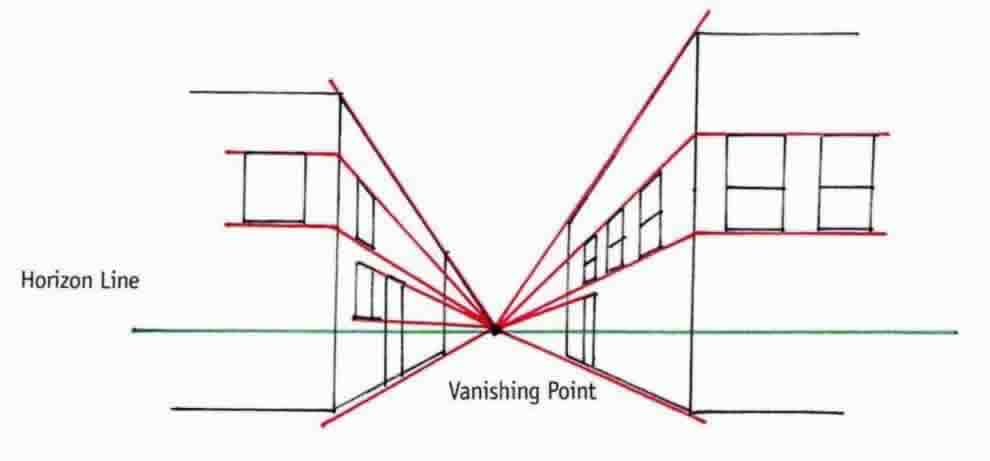
\includegraphics[width=10cm, height=5cm]{images/vanishing_point.jpg}%
  \caption{Example image of Vanishing Point}
\end{figure}

\end{frame}


\subsection{Architecture}
\begin{frame}{Design Architecture}

\begin{columns}[c]
    \column{0.4\textwidth}
        Architecture consists of 5 main components:
  \begin{itemize}
    \setlength\itemsep{1em}
    \item Parrot AR Drone Platform
    \item AR Drone SDK
      \begin{itemize}
	\item provides APIs to communicate with AR drone. 
      \end{itemize}
    \item Autonomy Driver(ROS Package)%\footnote[1]{Ardrone\_autonomy package can be downloaded from github. \textcolor{blue}{Git source :} \url{https://github.com/AutonomyLab/ardrone_autonomy.git} (branch hydro-devel).}
      \begin{itemize}
	\item interface between ROS and the AR.Drone(navigation messages, video feeds and control commands)  
      \end{itemize}
    \item Image Processing*
    \item Controller*
  \end{itemize}
        
    \column{0.6\textwidth}
        \begin{figure}
             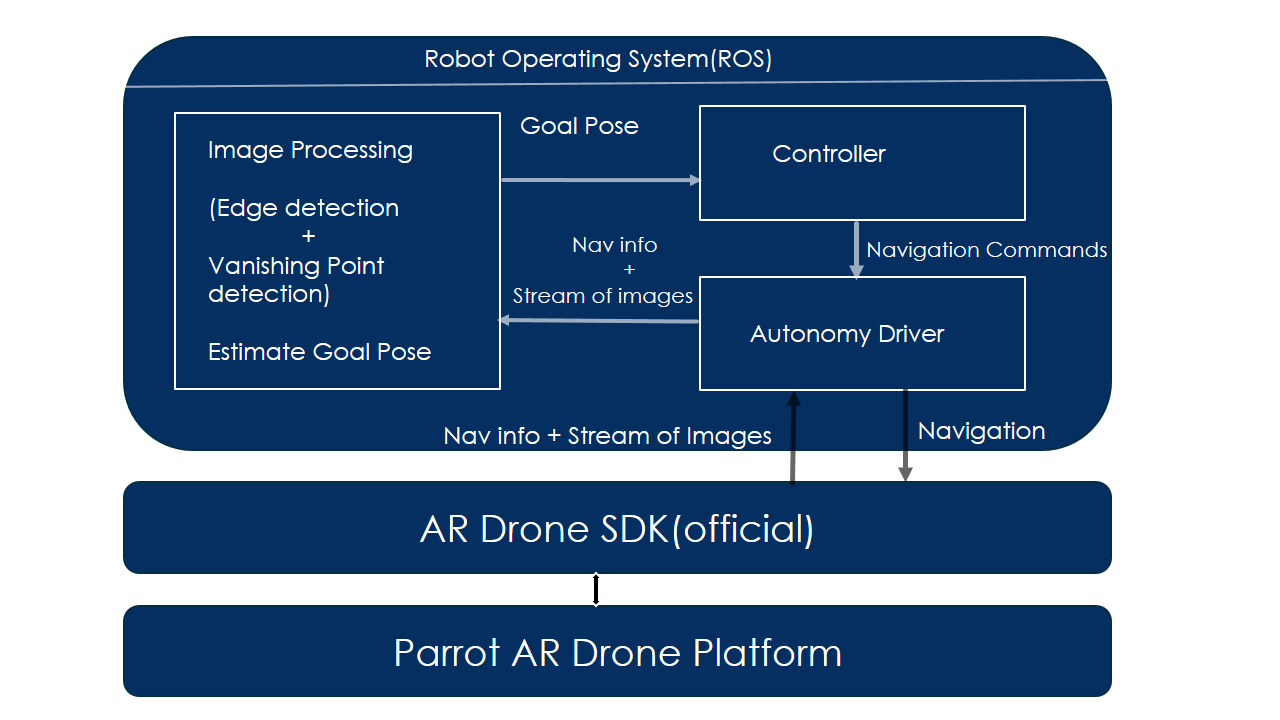
\includegraphics[width=8cm, height=7cm]{images/architecture.png} 
	     \caption{Component view of the Architecture}
        \end{figure}     
	 
\end{columns}

\end{frame}

\subsection{Image Processing}
\begin{frame}{Image Processing}
Detect vanishing point from the perspective cues from stream of images received through AR Drone.

\vspace{0.5cm}
Implemented two methods of detecting vanishing point:\vspace{0.3cm}
\begin{enumerate}
  \setlength\itemsep{1em}
  \item Classical VP based on edge detection
    \begin{itemize}
     \item straight lines extraction from images
    \end{itemize}
  \item VP based on image density clustering
    \begin{itemize}
     \item lines those move away from us converge towards the center of the picture.
    \end{itemize}
\end{enumerate}

\end{frame}

\begin{frame}<1>[label=vp_edge_detect]{Method 1: Classical approach based on edge detection}
Detecting the parallel lines in the environment is the premise for calculating the vanishing point.
\vspace{0.3cm}
Procedure for VP detection:
\begin{enumerate}
  \setlength\itemsep{1em}
  \item \alert<2>{Straight lines extraction}
  \begin{enumerate}
    \setlength\itemsep{1em}
    \item \alert<2>{preprocessing of image}
    %\item \color<2>{gray}\alert<3>{deleting noise interference}
    \item \color<2>{gray}\alert<3>{edge extracting using Canny operator}
    \item \color<2-3>{gray}\color<5>{black}\alert<4>{extracting lines by PHT(Probabilistic Hough Transform)}
  \end{enumerate}
 \item \color<2-3-4>{gray}\color<6>{black}\alert<5>{Deleting unreasonable straight lines}
 \item \color<2-3-4-5>{gray}\color<7>{black}\alert<6>{Locating vanishing point}
\end{enumerate}

\end{frame}

\againframe<2>{vp_edge_detect}

\begin{frame}{Preprocessing of image}
\begin{itemize}
  \setlength\itemsep{1em}
 \item Enhance image for more understandable level of feature extraction (Gray scale conversion).
 \item Smoothen the image to reduce noise (Normalized Box filter\footnote{Each output pixel is the mean of its kernel neighbors ( all of them
contribute with equal weights).})
\end{itemize}

\end{frame}

\againframe<3>{vp_edge_detect}


\begin{frame}{Output of Canny operator}
 \begin{figure}
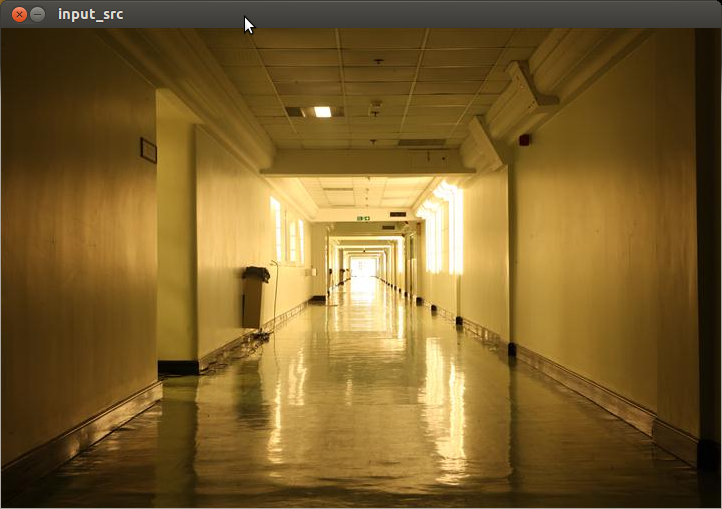
\includegraphics[width=6cm, height=5cm]{images/inputimage.png}%
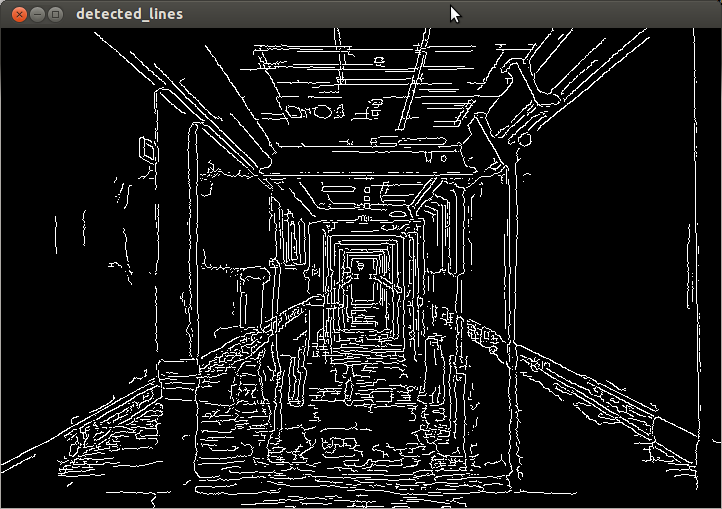
\includegraphics[width=6cm, height=5cm]{images/detected_edges.png}%
\caption{Detected edges using canny edge detector}%
\label{fig:detectedegdes}
\end{figure}
\end{frame}


\againframe<4>{vp_edge_detect}

\begin{frame}{Output of Probabilistic Hough Transform}
 \begin{figure}
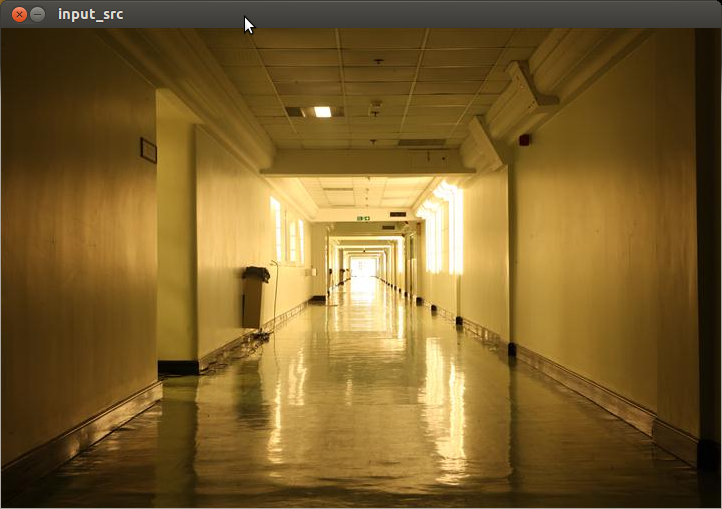
\includegraphics[width=6cm, height=5cm]{images/inputimage.png}%
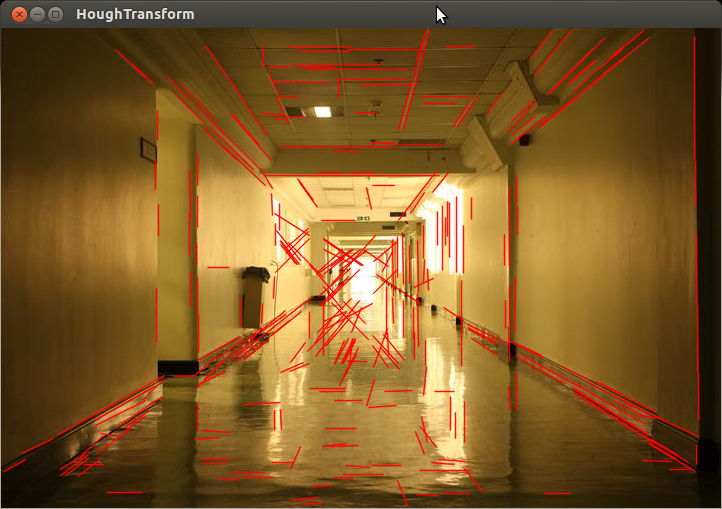
\includegraphics[width=6cm, height=5cm]{images/Hough_Lines.png}%
\caption{Results of Hough Line Transform}%
\end{figure}
\end{frame}

\againframe<5>{vp_edge_detect}

\begin{frame}{Deleting unreasonable straight lines}
 \begin{itemize}
  \setlength\itemsep{1em}
  \item Detected lines from Hough Transform include vertical and horizontal edges. 
  \item These lines do not converge to VP, hence not useful. 
  \item Such lines are filtered in order to have a more accurate VP detection. 
  \item Lines which have slope between $\theta_1 = \pm10^{\circ}$ or $\theta_2 = \pm10^{\circ}$ are deleted.
 \end{itemize}
 \begin{figure}
 \centering
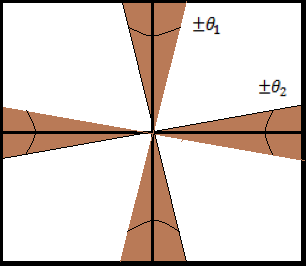
\includegraphics[width=3cm, height=3cm]{images/deleted.png}%
\caption{Unreasonable lines with slope between $\theta_1 = \pm10^{\circ}$ and $\theta_2 = \pm10^{\circ}$}%
\label{fig:unreasonablelines}
\end{figure}

\end{frame}

\againframe<6>{vp_edge_detect}

\begin{frame}{Locating vanishing point}	
\begin{enumerate}
\setlength\itemsep{1em}
 \item divide the image plane into a 22 x 33 grid G
 \item calculate all intersections of the lines obtain from RHT
 \item calculate the number of lines intersection falling in each grid element $G(x,y)$
 \item consider $G(a,b)$ number of intersection lines falling in each grid element where $a \in [0,22)$ and $b \in [0,33)$.
\end{enumerate}\\[5pt]
\hspace{3mm}The grid with the maximum number of intersections is:\\[5pt]
{\centering  (a^*,b^*) = \texttt{argmax}_{ab} G(a,b)\par}\\[5pt]
\hspace{3mm}and vanishing point is given as:\\[5pt]
{\centering (x_{vp},y_{vp}) = ((a^{*}+0.5)*w/33,(b^{*}+0.5)*h/22) \\[5pt] 
w,h - width,height of image\par}
\end{frame}

\begin{frame}{Locating vanishing point}	
 Left figure shows division of image into a grid of $22 \times 33$ and right figure displays result of extracted vanishing point using edge detection method.\\[5pt]
\begin{figure}
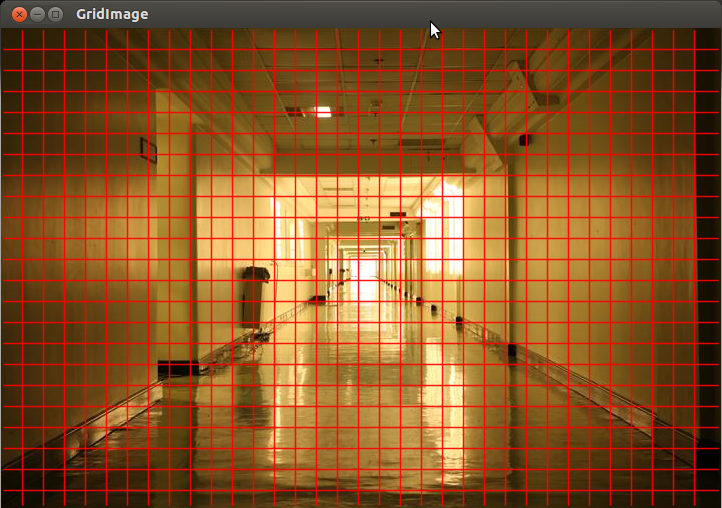
\includegraphics[width=6cm, height=5cm]{images/gridimage.png}%
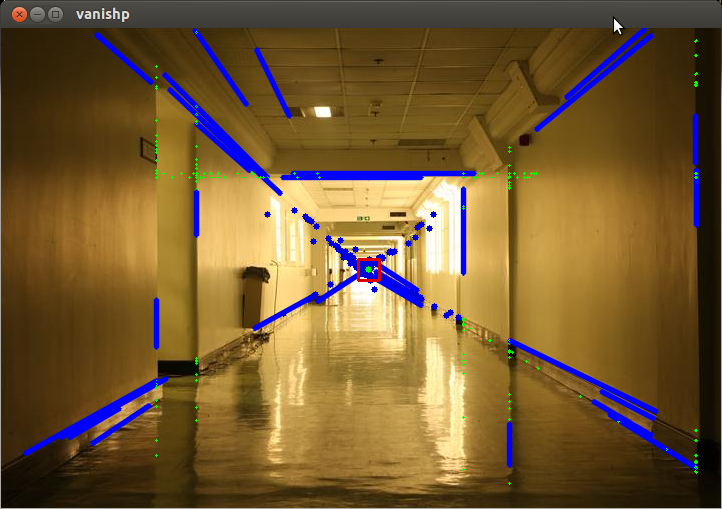
\includegraphics[width=6cm, height=5cm]{images/vanishingpointss.png}%
\caption{Divided image into a $22 \times 33$ grid and located vanishing point}%
\label{fig:gridimage}
\end{figure}
\end{frame}



\iffalse{
%%%%%%%%%%%%%%%%%%%
{
\begin{frame}<1-3>[label=longthing]
     \frametitle{Scenario}
     \begin{itemize}<+->
         \item Foo
         \item Bar
         \item Baz
         \item Boo
         \item Far
         \item Zab
     \end{itemize}
\end{frame}

\begin{frame}
     \frametitle{Explainatory Frame}
     To explain these three points (Foo, Bar, Baz):
     \begin{itemize}[<+->]
         \item Foo is good
         \item Bar is bad
         \item Baz is ugly
     \end{itemize}
\end{frame}

\againframe<4-6>{longthing}
%%%%%%%%%%%%%%%%%%%%%%%%%%%%%%%%%%%55


\begin{frame}<1>[label=again]
  \frametitle{The Infamous Disappearing Text}

Here is a frame, it's a bit \alert<2-3>{boring}.

It's so boring, we'll see it \only<-3>{{\color<2-3>{gray}twice}}.

\only<3>{But the second time, we'll try to make it more interesting by making some of those words change colour.}

\only<5>{The third time, we'll wave a magic wand to make all the gray words disappear.}

\end{frame}

\begin{frame}
\frametitle{Some Comments}
This frame is perhaps even more so.
\end{frame}

\againframe<2-3>{again}

\begin{frame}
\frametitle{Some Comments}
Will this tedium ever end?
\end{frame}

\againframe<4-5>{again}


\fi

\begin{frame}<1>[label=vp_density_based]{Method 2: VP based on image density clustering}
\color[rgb]{0.59, 0.0, 0.09}\textit{Density of points of intersection of lines is maximum towards the center.}
Procedure for VP detection:
  \begin{enumerate}
    \setlength\itemsep{1em}
    \item \alert<2>{preprocessing of image}
    %\item \color<2>{gray}\alert<3>{deleting noise interference}
    \item \color<2>{gray}\alert<3>{locate vanishing point}
    %\item \color<2-3>{gray}\color<5>{black}\alert<4>{integral image to find densities}
  \end{enumerate}

\end{frame}

\againframe<2>{vp_density_based}

\begin{frame}{Preprocessing of image}
\begin{itemize}
  \setlength\itemsep{1em}
 \item convert the image in to grayscale
 \item apply the Sobel operator in both x and y direction to find out the edges.
\end{itemize}
\begin{figure}
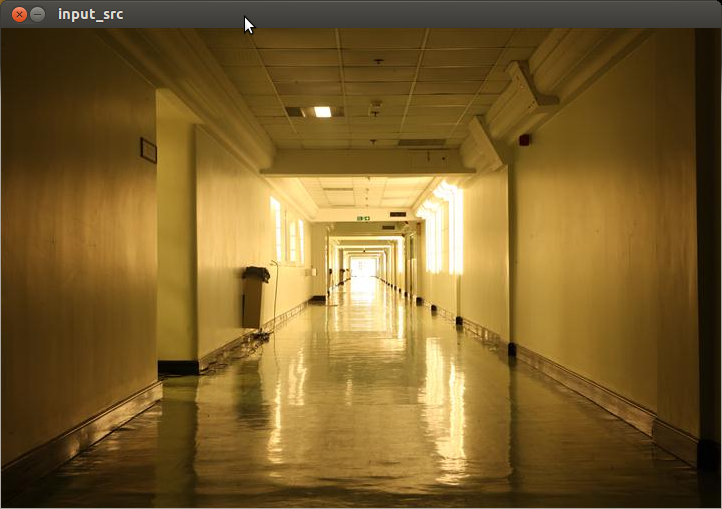
\includegraphics[width=6cm, height=5cm]{images/inputimage.png}%
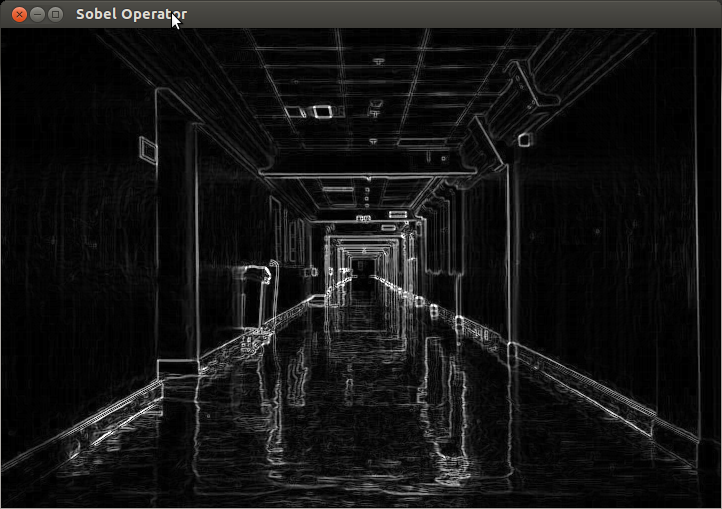
\includegraphics[width=6cm, height=5cm]{images/sobelop.png}%
\caption{Output of sobel operator}%
\end{figure}
\end{frame}

\againframe<3>{vp_density_based}

\begin{frame}{Locate vanishing point}

{ \color[rgb]{0.59, 0.0, 0.09}{\textit{VP is the point of maximum density, the aim is to find that point.}}}\\[5pt]

Procedure:\\[5pt]
\begin{itemize}
\setlength\itemsep{1em}
\item Take a square box of side size equal to the one smaller between height(h) and width(w)
 \item Scroll through the image from left to right if w \textgreater h else top to bottom
 \item Keep track of density of points in each box and after the complete scroll, take the box with maximum density
 \item Repeat the process for 25 times and each time the scrolling area is reduced to the box selected from the last scroll.
\end{itemize}
\iffalse{
\begin{algorithm}[H]
\caption{VP based on image density}\label{euclid}
\begin{algorithmic}
        \Function{vp\_detection}{image sobel\_image, int iterations}
            \State $w \gets $ \textit{width of image}
            \State $h \gets $ \textit{height of image}
            \If{$ w < h$}
                \State $side\_size \gets $ \textit{w-1}
                %\State $sq\_side \gets h$ 
            \EndIf
            \If{$ h < w$}
                %\State $scoll\_direction \gets $ \textit{top\_to\_bottom}
                %\State $no\_of\_scroll \gets $ \textit{h}
                \State $side\_size \gets $ \textit{h-1}
                %\State $sq\_side \gets w$ 
            \EndIf
	      %\State $prev\_ysize \gets s.height$
	      %\State $prev\_xsize \gets s.width$
	      %\State $pxx \gets$ 1
	      %\State $pyy \gets$ 1
	      %\State $density \gets$ 0
            \ForAll{$i$ in $iterations$}
	      %\State $max\_density \gets$ 0;
	      %\State $y_limit \gets pyy+prev\_ysize-1-side\_size$
	      %\State $x_limit \gets pxx+prev\_xsize-1-side\_size$
	      \While{$y < y\_limit$} 
	      %\While{$x < x\_limit$}
	      %\State $densities[j] \gets image\_density(x,y)$
	      %\State $ \gets image\_density(x,y)$
	      %\State $densities[j] \gets image\_density(x,y)$
	      \EndWhile
	      \EndWhile
                \Repeat 
                    \State $densities[j] \gets image\_density(x,y)\\
                    \Call{Scroll}{x,y}
                \Until{$j \neq no\_of\_scroll$}
	      \State $x,y \gets max\_density\_xy(densities)$\\
	      $\Call{shrink}{x,y}$
	    \EndFor 
        \EndFunction
    \end{algorithmic}
\end{algorithm}
}
\fi

\end{frame}

\begin{frame}{Locating vanishing point}
 \begin{figure}
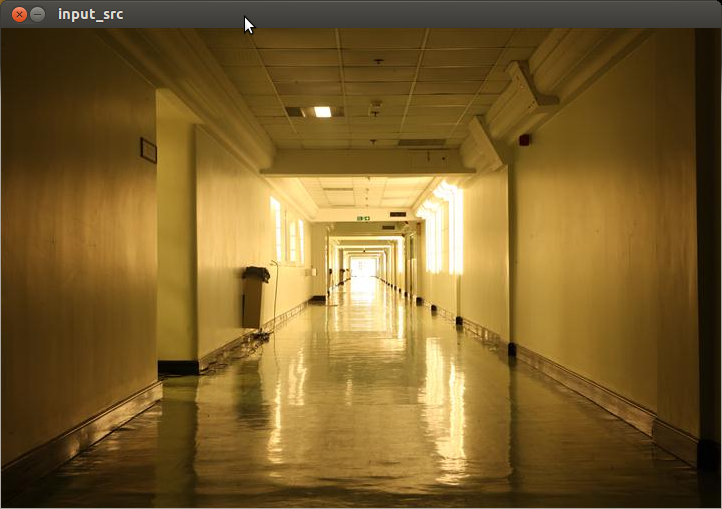
\includegraphics[width=6cm, height=5cm]{images/inputimage.png}%
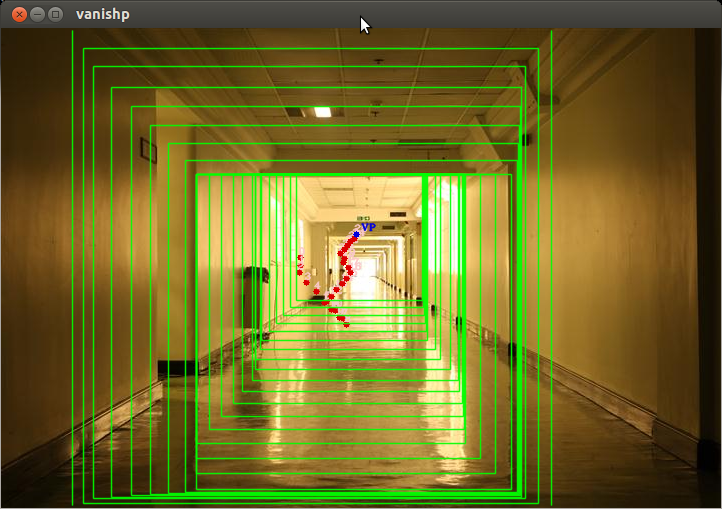
\includegraphics[width=6cm, height=5cm]{images/densityop.png}%
\caption{Output of density based vanishing point}%

\end{figure}
\end{frame}

\begin{frame}{Integral image to find densities}
\begin{itemize}
\setlength\itemsep{1em}
 \item Calculating intensity of each pixel in a box and summing them is a time consuming process. 
 \item Integral image helps to rapidly calculate summations over image subregions
 \item Every pixel in an integral image is the summation of the pixels above and to the left of it. 
 \item We can construct the integral image of a given image with only one pass over the given image. 
\end{itemize}\\[5pt]
Value $s$ of a pixel $(x,y)$ in output image is : \\[2pt]
%{\centering  $s(x,y) = i(x,y) + s(x-1,y) + s(x,y-1) + s(x-1,y-1)$\par}\\[2pt]
\begin{equation*}
 s(x,y) = i(x,y) + s(x-1,y) + s(x,y-1) + s(x-1,y-1)
\end{equation*}

 \begin{figure}
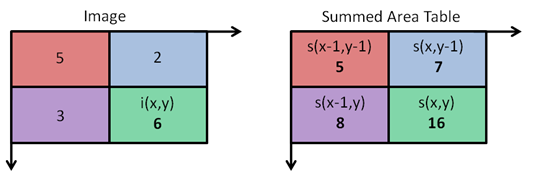
\includegraphics[width=6cm, height=2cm]{images/integralimage.png}%
\caption{Integral image concept}%
{\small \color{gray}{[Photo credit: https://computersciencesource.wordpress.com]}}
\end{figure}
\end{frame}

\begin{frame}{Integral image to find densities}
 \begin{figure}
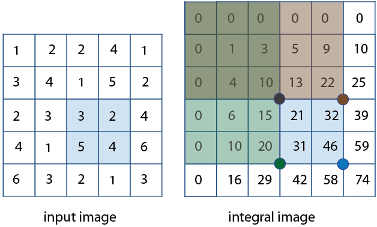
\includegraphics[width=6cm, height=3cm]{images/integral_image_b.png}%
\caption{Example of integral image}%
{\small \color{gray}{[Photo credit: https://www.mathworks.com]}}
\end{figure}\\[5pt]
To calculate density of any sub region in image, we need only 4 values. This process have now $O(1)$ complexity.
\begin{equation*}
 i(x\prime,y\prime) = s(\texttt{left top}) + s(\texttt{bottom right}) - s(\texttt{top right}) - s(\texttt{bottom left})
\end{equation*}
\end{frame}


\begin{frame}{Edge detection Vs Image density clustering}
\begin{itemize}
\setlength\itemsep{1em}
 \item VP detection based on image density is faster than edge detector method 
 \item \alert{But very sensitive in case of noise or obstacles in the environment}
 \item Therefore, we used VP detection based on edge detection.
\end{itemize}\\[5pt]
\begin{figure}
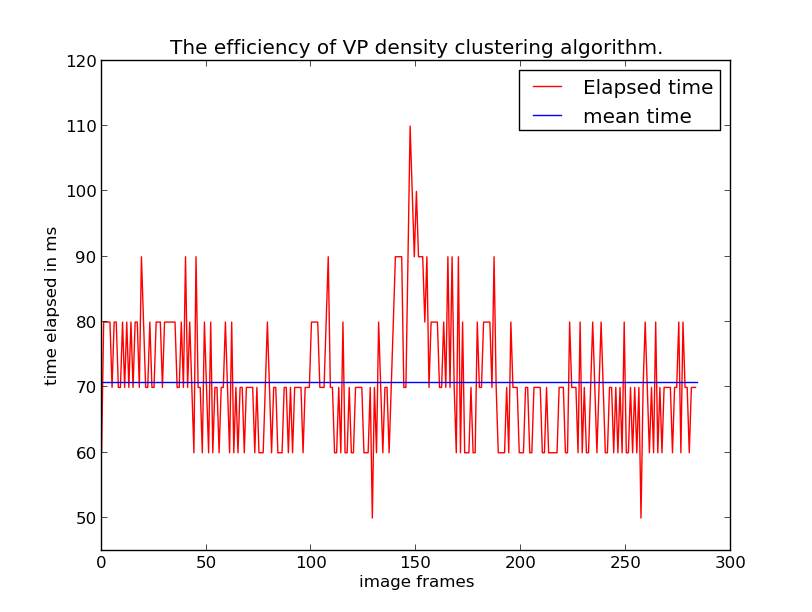
\includegraphics[width=6cm, height=4cm]{images/Elapsedtimeedgedetection.png}%
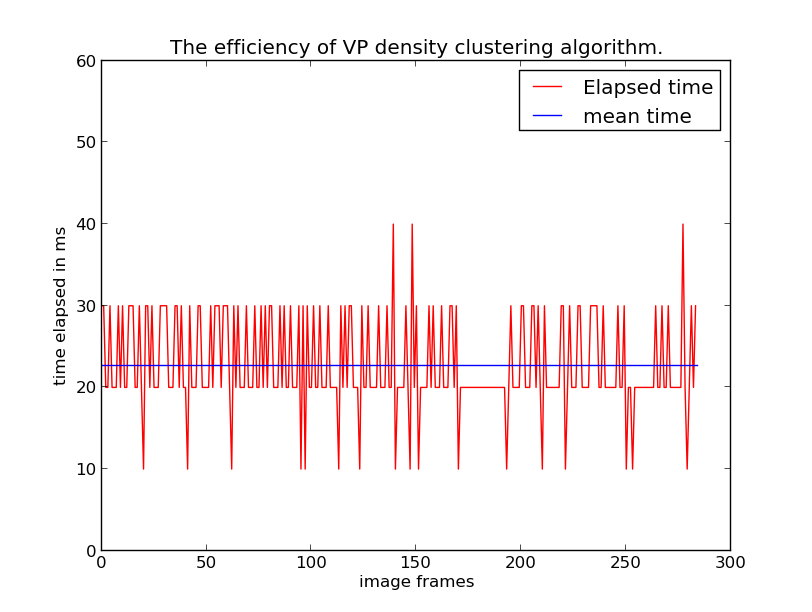
\includegraphics[width=6cm, height=4cm]{images/Elapsedtimedensity.png}%
\caption{Time elapse by Edge detector method (left) and Density cluster(right) over 250 sample images}%
\end{figure}
\end{frame}
\begin{frame}{Reliability of Vanishing Point detected}
\begin{itemize}
\setlength\itemsep{1em}
 \item Keep track of vanishing point detected in previous frame
 \item Resultant vanishing point is the latest vanishing point detected half plus previous vanishing point half. 
\end{itemize}\\[5pt]
\begin{equation*}
 (x_{vp},y_{vp}) = (current_{vp}.x/2 + previous_{vp}.x/2, current_{vp}.y/2 + previous_{vp}.y/2)
\end{equation*}\\[5pt]
{ \color[rgb]{0.59, 0.0, 0.09}{\textit{This can be further optimized by keeping track of last few output points and calculate average of all previous and latest detected point as the output of the current frame.}}}

\end{frame}

\subsection{Controller}
\begin{frame}{Controller}
\begin{itemize}
\setlength\itemsep{1em}
 \item Controller receives estimated pose from image processing module and sends flight commands to the AR.Drone via ardrone autonomy.
 \item Aim to maintain at zero, the horizontal distance between the vanishing point and the center of the image. 
 \item PID controller is used in our approach to directly control the quadrocopter.
 \begin{itemize}
  \item \textbf{P}: helps to reduce the error
  \item \textbf{I}: helps to maintain the stable state(hold state)
  \item \textbf{D}: damps occurring oscillations
 \end{itemize}
\item Separate controller for yaw angle and command velocities
\end{itemize}\\[5pt]

\end{frame}

\begin{frame}{Controller}
 \begin{figure}
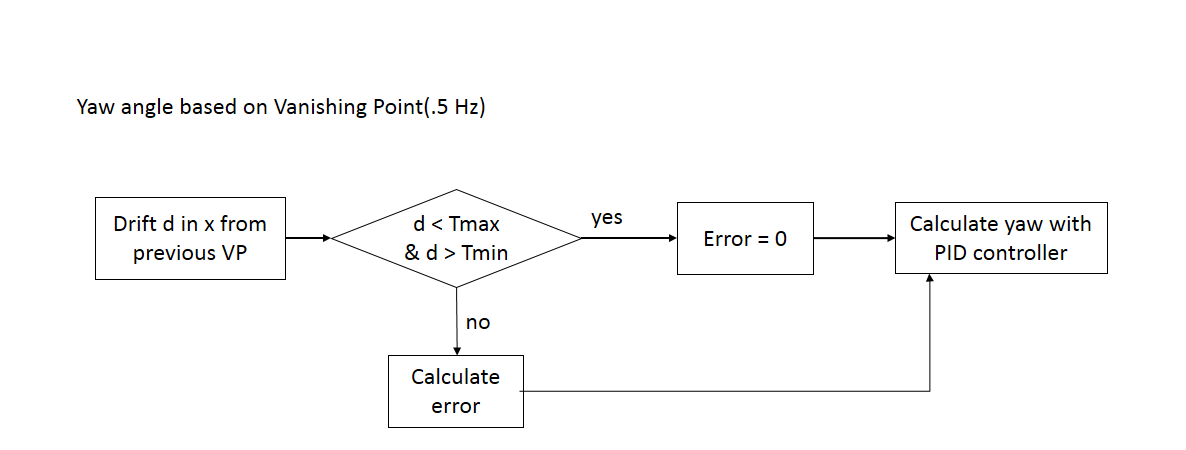
\includegraphics[width=10cm, height=3cm]{images/Yaw_controller.png}%
\caption{Controller for yaw angle}%
\end{figure}
\vspace{0.3cm}
\begin{figure}
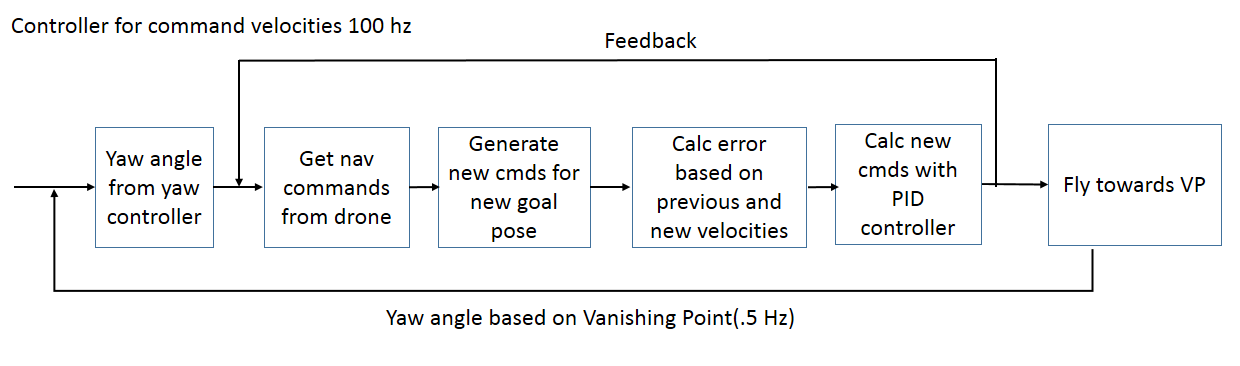
\includegraphics[width=10cm, height=3cm]{images/cmd_controller.png}%
\caption{Controller for navigation commands}%
\end{figure}
\end{frame}

\begin{frame}{Controller}
\begin{itemize}
\setlength\itemsep{1em}
 \item Vanishing point auto mode can be suppressed by joystick mode.
\end{itemize}\\[5pt]
{\centering State diagram of the drone\par}
\begin{figure}
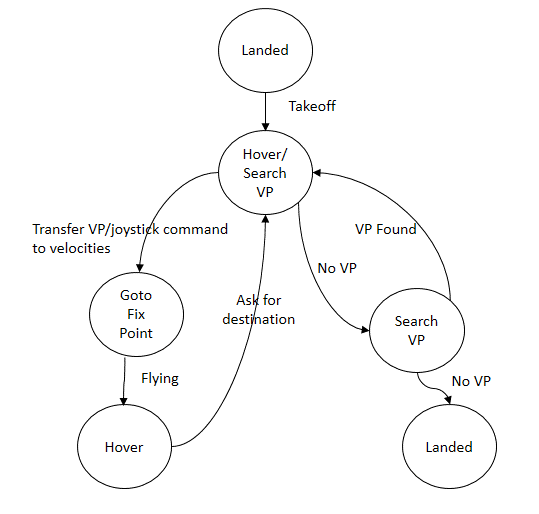
\includegraphics[width=6cm, height=5cm]{images/Statediagram1.png}%
\caption{State diagram of drone}
\end{figure}

\end{frame}

\section{Experimental results}
%\subsection{Experimental results}
\begin{frame}{Experimental results}
 Tested our approach in several corridors such as narrow, broad, corridors with obstacles and dark corridors.\\[2pt]
\begin{itemize}
 \item Accuracy of vanishing point detection approach
\end{itemize}
\vspace{0.3cm}
%{\centering \textit{Variance in VP position}\par}
\begin{columns}
 \column{0.5\textwidth}
  {\centering \small{\textit{with sharp maneuvers}\par}}
  \begin{figure}
  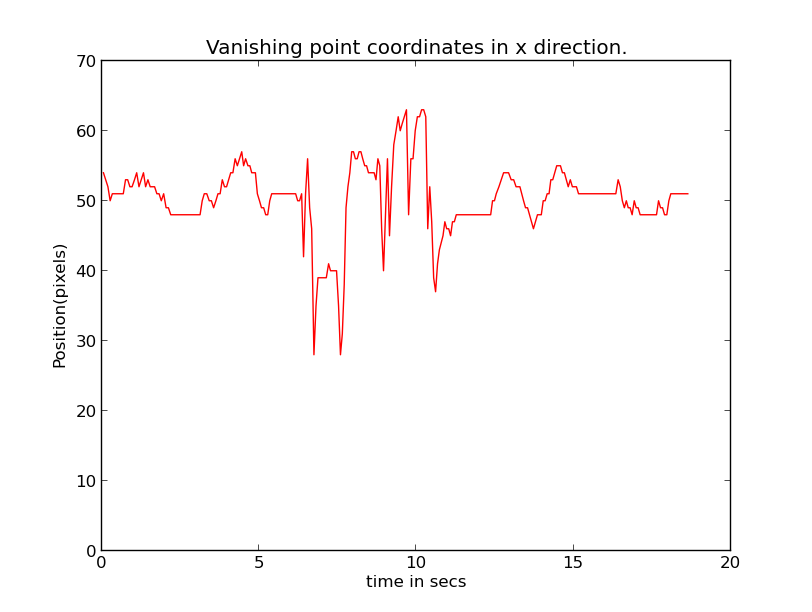
\includegraphics[width=5cm, height=3cm]{images/vpRobustness1a.png}
  %\caption{with sharp maneuvers}
  \end{figure}
 \column{0.5\textwidth}
  {\centering \small{\textit{without sharp maneuvers}\par}}
  \begin{figure}
   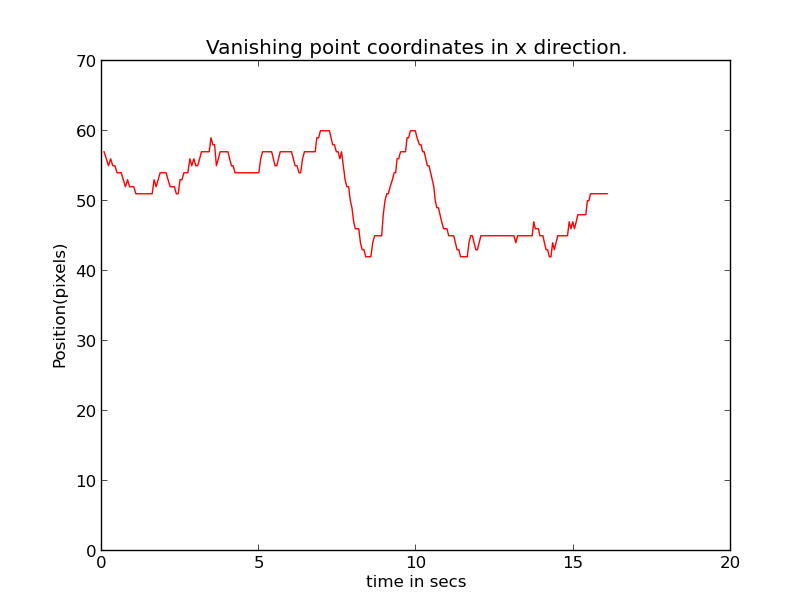
\includegraphics[width=5cm, height=3cm]{images/vpRobustness2a.png}
   %\caption{without sharp maneuvers}
   \end{figure}
\end{columns}\\[2pt]
{\centering \small{\textit{Dark Corridor(bad illumination)}\par}}
\begin{figure}
%\caption{[Dark Corridor(bad illumination)}
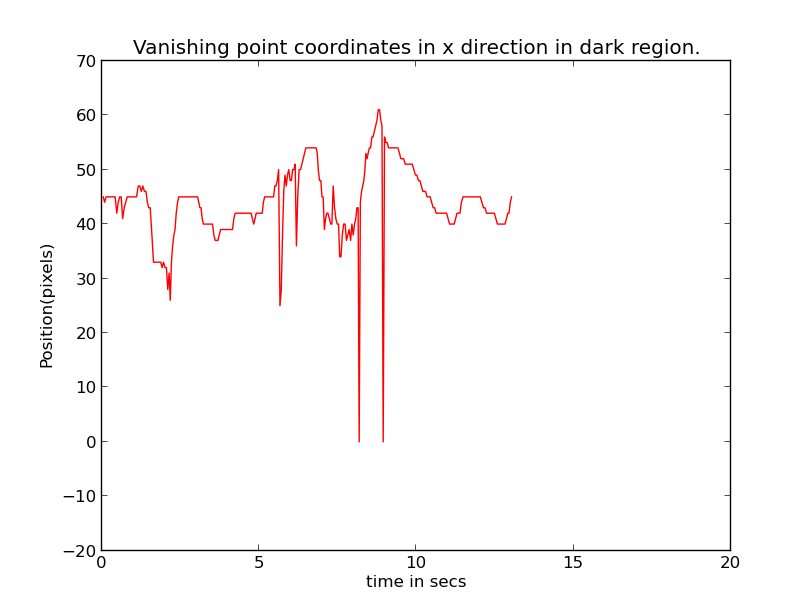
\includegraphics[width=5cm, height=2.5cm]{images/vpinDarkfloor.png}
%\caption{[Dark Corridor(bad illumination)}
\end{figure}%
%\caption{Variance in VP position}
%\label{fig:vpvariance} %% label for entire figure
%\end{figure}

\end{frame}


\begin{frame}{VP Evaluation}
\begin{itemize}
 \item Different corridors for VP testing
\end{itemize}
Current system does not consider obstacles if there are enough lines to calculate the vanishing point\\
%{\centering \textit{Variance in VP position}\par}
\vspace{0.5cm}
\begin{columns}
 \column{0.5\textwidth}
  {\centering \small{\textit{Dark corridor example}\par}}
  \begin{figure}
  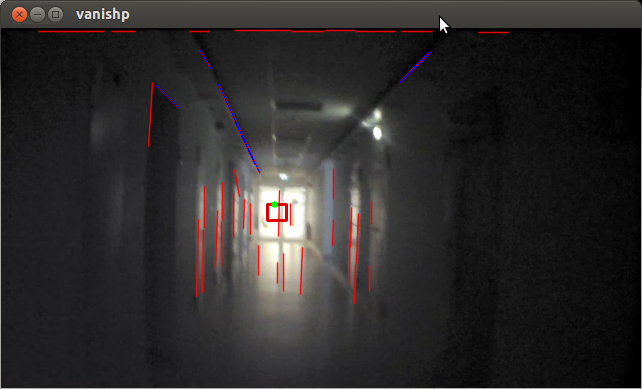
\includegraphics[width=6cm, height=5cm]{images/darkcorridor.png}
  %\caption{with sharp maneuvers}
  \end{figure}
 \column{0.5\textwidth}
  {\centering \small{\textit{VP with obstacle}\par}}
  \begin{figure}
   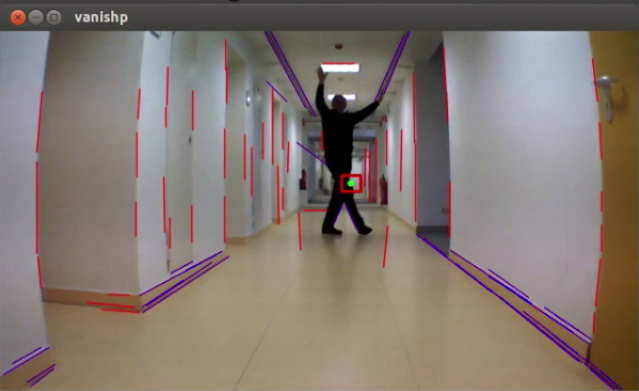
\includegraphics[width=6cm, height=5cm]{images/VPwithobstacle.png}%
   %\caption{without sharp maneuvers}
   \end{figure}
\end{columns}
\end{frame}

\begin{frame}{Controller Evaluation}
We evaluated controller based on the variation in Linear $x$ (horizontal) ,Linear $y$ (vertical) and angular $z$ (yaw) velocities \\[5pt]
\vspace{0.3cm}
\begin{columns}
 \column{0.6\textwidth}
  {\centering \small{\textit{Linear roll and pitch velocities on real flight}\par}}
  \begin{figure}
  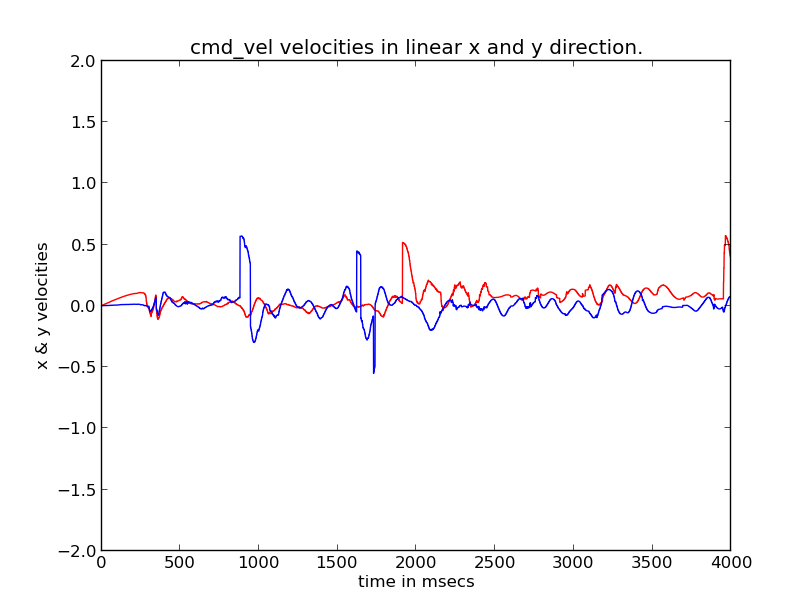
\includegraphics[width=6cm, height=4cm]{images/cmdxy2.png}%
  %\caption{with sharp maneuvers}
  \end{figure}
 \column{0.4\textwidth}
  {\centering \small{\textit{Linear $X Y Z$ axis}\par}}
  \begin{figure}
   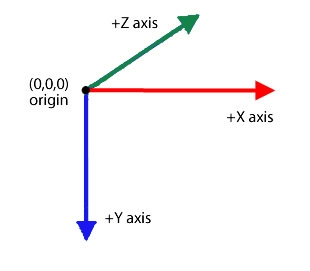
\includegraphics[width=3cm, height=3cm]{images/xyzAxes.jpg}%
   %\caption{without sharp maneuvers}
   \end{figure}
\end{columns}
%{\centering \textit{Variance in VP position}\par}
\end{frame}

\begin{frame}{Controller Evaluation}
Variation in  yaw angle shows the robustness of the controller \\[5pt]
\begin{figure}
  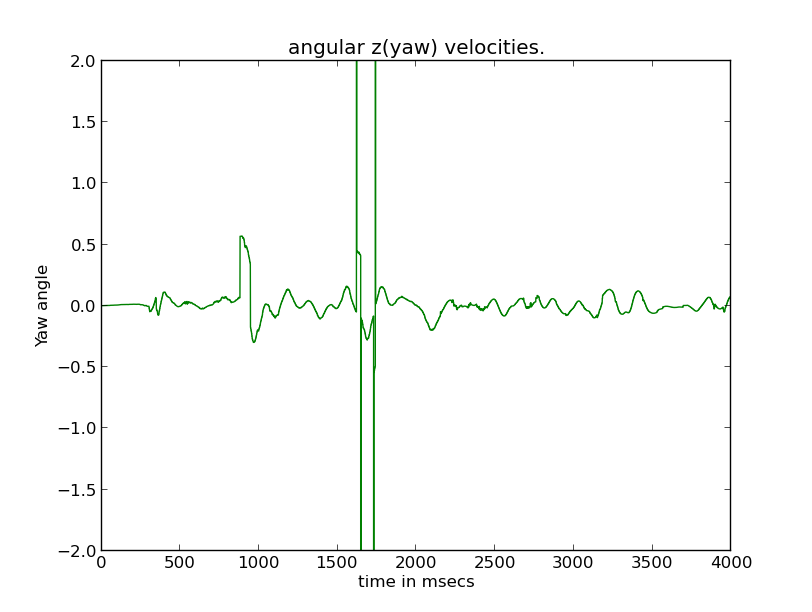
\includegraphics[width=10cm, height=4cm]{images/angularyaw.png}%
  \caption{Angular velocities of the drone during flight} 
  \label{fig:cmdxy}%
\end{figure}
%{\centering \textit{Variance in VP position}\par}
\end{frame}
% Placing a * after \section means it will not show in the
% outline or table of contents.

\section{Future work}

\begin{frame}{Future work}
  \begin{itemize}
  \setlength\itemsep{1em}
  \item
    \textbf{Density based VP detection} is promising and less computationally expensive. Can be improved for useful VP based navigation 
  \item \textbf{Edge based VP detection:} Vanishing point is sometimes found on the edge which is not accepted for drone to fly. This needs to be improved and made more reliable. 
  \item
    \textbf{Onboard Computation:} Currently algorithm works on host machine, still need to be implemented on Asctec Pelican. 
  \end{itemize}
\end{frame}

% All of the following is optional and typically not needed. 
%\appendix
%\section<presentation>*{\appendixname}
%\subsection<presentation>*{For Further Reading}
\section*{Appendix}
\subsection{videos}
\begin{frame}
 %{\centering THANK YOU \par}
 \begin{center}
  \Large {VIDE{\Laughey}S}
 \end{center}
\end{frame}
\end{frame}

\subsection{References}
\begin{frame}{References}
    
  \begin{thebibliography}{10}
  % Start with overview books.
  \bibitem{1} B. Ajith Kumar and D. Ghose, Radar-assisted collision avoidance, guidance strategy for planar flight, Aerospace and Electronic Systems, IEEE Transactions on, vol. 37, pp. 77-90, Jan 2001.
  \bibitem{2} Y. Kwag and J. Kang, Obstacle awareness and collision avoidance radar sensor system for low-altitude flying smart uav, Digital Avionics Systems Conference, 2004. DASC 04. The 23rd, vol. 2, pp.12.D.2,121-10 Vol.2, 24-28 Oct. 2004. 
  \bibitem{3} Saunders, O. Call, A. Curtis, A. W. Beard, and T. W. Mclain, Static and dynamic obstacle avoidance in miniature air vehicles, in Proceedings of the Infotech@Aerospace Conference, pp. 2005-6950, 2005.
  \bibitem{4}J. Courbon, Y. Mezouar, N. Guenard, and P. Martinet, Visual navigation
of a quadrotor aerial vehicle, in IROS, 2009.
  \bibitem{5} Haiyang Chao; Yu Gu; Napolitano, M., "A survey of optical flow techniques for UAV navigation applications," Unmanned Aircraft Systems (ICUAS), 2013 International Conference on , vol., no., pp.710,716, 28-31 May 2013
  \bibitem{6} G. Conte and P. Doherty  "Vision-based unmanned aerial vehicle navigation using georeferenced information",  EURASIP J. Adv. Signal Process.,  vol. 2009,  pp.10 2009 
  %\bibitem{3} Bills, C. ; Chen, J. ; Saxena, A., "Autonomous MAV flight in indoor environments using single image perspective cues", Robotics and Automation (ICRA), 2011 IEEE International Conference on 9-13 May 2011, pages = 5776 - 5783.
  %\bibitem{4}F. Schaffalitzky and A. Zisserman, “Planar grouping for automatic detection of vanishing lines and points,” Image and Vision Computing, vol. 18, no. 9, pp. 647–658, 2000.
  \end{thebibliography}
\end{frame}

\begin{frame}
 %{\centering THANK YOU \par}
 \begin{center}
  \Large {\underline{THANK Y{\Laughey}U}}\\[5pt]
 \normalsize{ Devvrat Arya\\
  \textit{devvrat.arya@smail.inf.h-brs.de}}
 \end{center}
\end{frame}

\subsection{Edge detection}
\begin{frame}{Edge extracting using Canny operator}
 Canny Edge detector -  optimal Edge detector %with low error rate and good localization.
 %\vspace{0.2cm}This includes 4 procedures:
 \begin{itemize}
 \setlength\itemsep{1em}
  \item Gaussian Filter De-noising
  \item Gradient Operator Sobel\\ \small{
	Finds the intensity gradient of the image in vertical and horizontal direction using Sobel Operators.\\
	%Takes gradient of the image in the horizontal and vertical directions with Sobel operators\\
	\begin{center}
  $G_x = \begin{bmatrix}
      -1 & 0 & +1\\
      -2 & 0 & +2\\
      -1 & 0 & +1
      \end{bmatrix} , \qquad 
      G_y = \begin{bmatrix}
      -1 & -2 & -1\\
       0 &  0 &  0\\
      +1 & +2 & +1
      \end{bmatrix}$\\
      \end{center}
      The magnitude $|\bar{G}|$ and orientation $\theta$ of the image gradient are thus given by: \\[2pt]
   {\centering
   \|\bar{G}(x,y)\| = \sqrt{{\bar{G}_x}^2 + {\bar{G}_y}^2} ,\qquad   
    \theta = \texttt{arctan}\left( \frac{\bar{G}_y}{\bar{G}_x}\right)
  \par}}
  \item Control of Gradient Value\\
	\small{Suppress any pixel value (i.e. set it equal to zero) that is not considered to be an edge.}
  \item Hysteresis\\
	\small{Track along the remaining pixels that have not been suppressed.}
 \end{itemize}

\end{frame}

\begin{frame}{Extracting lines by PHT(Probabilistic Hough Transform)}
%Randomized or Probabilistic Hough Transformation (PHT) is one of the most commonly used algorithms in perspective vision. \\
\begin{itemize}
 \item The algorithm is based on the parametric representation of a line:\\[5pt]
  {\centering \rho = x\cos \theta + y\sin \theta\par}\\[5pt]
  %\end{center}\\
where $\rho$ is perpendicular distance from the origin to the line and $\theta$ is angle between horizontal axis and this perpendicular.
\item Family of lines that goes through a point $(x,y)$, gives a sinusoid.
\begin{columns}[c]
    \column{0.5\textwidth}
      \begin{figure}
      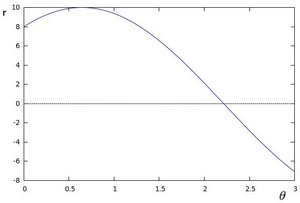
\includegraphics[width=4cm, height=3cm]{images/Hough_Lines_Tutorial_Theory_1.jpg}%
      \caption{$(\rho,\theta)$ plot for points $(x,y)$}%
      \label{fig:Hough_Lines_Tutorial_Theory}
      \end{figure}
    \column{0.5\textwidth}
     \begin{figure}
      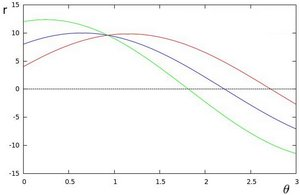
\includegraphics[width=4cm, height=3cm]{images/Hough_Lines_Tutorial_Theory_2.jpg}%
      \caption{$(\rho,\theta)$ plots for 3 points $(x,y)$ intersecting at one single point}%
      %[Photo credit: \href{http://docs.opencv.org/doc/tutorials/imgproc/imgtrans/hough_lines/hough_lines.html}{Opencv documentation Hough Line Transform}]
      \label{fig:sinusoidalIntersection}
      \end{figure}
\end{columns}
\item \color[rgb]{0.59, 0.0, 0.09}{\textit{Same operation is done for all the points in an image. If curves of two different points intersect in the plane $(\theta$ - $\rho)$, that means both points belong to a same line.}}
\end{itemize}
\end{frame}

\end{document}


